  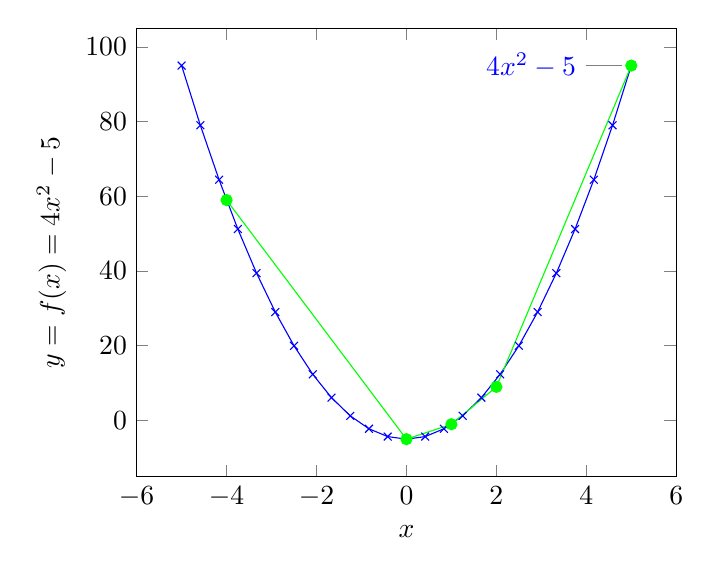
\begin{tikzpicture}
      \begin{axis}[           % das Koordinatensystem wird mit
                              % der Umgebung axis erzeugt,
                              % hier zusätzliche Optionen
            xlabel=\(x\),
            ylabel={\(y=f(x)=4x^2 - 5\)} % {...} wegen der
                              % Leerzeichen
          ]
          \addplot[           % ein Plot wird hinzugefügt
            domain=-5:5,      % der Definitionsbereich
            color=blue,
            mark=x            % berechnete Punkte werden mit
                              % einem x markiert
          ] { 4*x^2-5 }       % die Funktion
          node [pin=180:{$4x^2-5$}]{}; % Legende der Grafik
          \addplot[
            domain=-5:5,
            color=green,
            mark=*
          ]
          coordinates {
            (-4, 59)
            (0, -5)
            (1, -1)
            (2, 9)
            (5, 95)
          };
      \end{axis}
  \end{tikzpicture}
